\documentclass[]{standalone}

\begin{document}
	\begin{frame}{Brain Extraction}{Atlas registration, Brain normalization and Skull Stripping}
	
	\vspace{-25pt}
		\begin{columns}
			\begin{column}{0.45\textwidth}
				\begin{itemize}
				\item Atlas Registration;
				\item Normalization;
				\item Thresholding;
				\item Find the Largest Connected Component.
				\end{itemize}
			\end{column}
			\begin{column}{0.55\textwidth}
			\begin{figure}[h!]
			\centering
			\vspace{-6pt}
				\begin{subfigure}{0.45\textwidth}
					\centering
					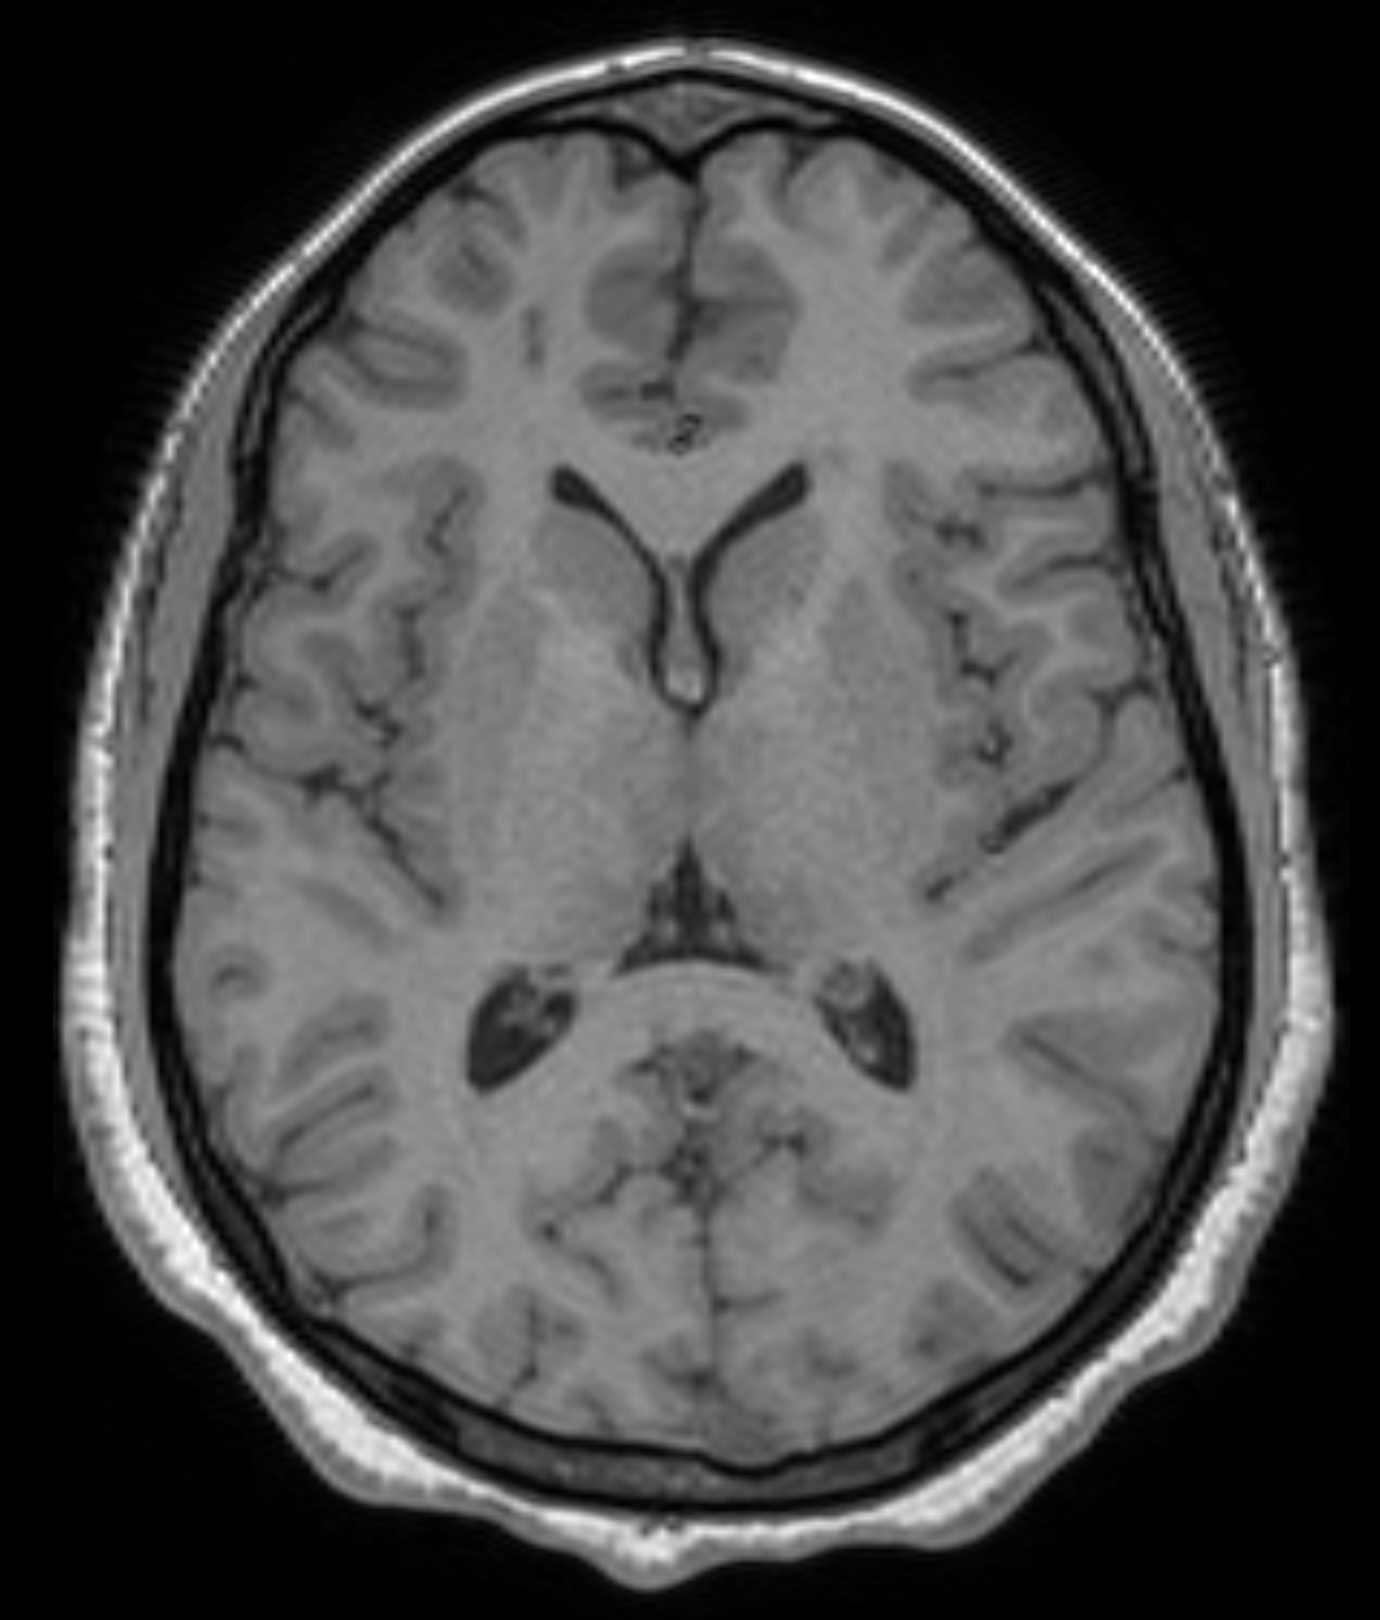
\includegraphics[scale=0.05]{./IMG/T1.jpg}
				\end{subfigure}
				\hfill
				\begin{subfigure}{0.45\textwidth}
					\centering
					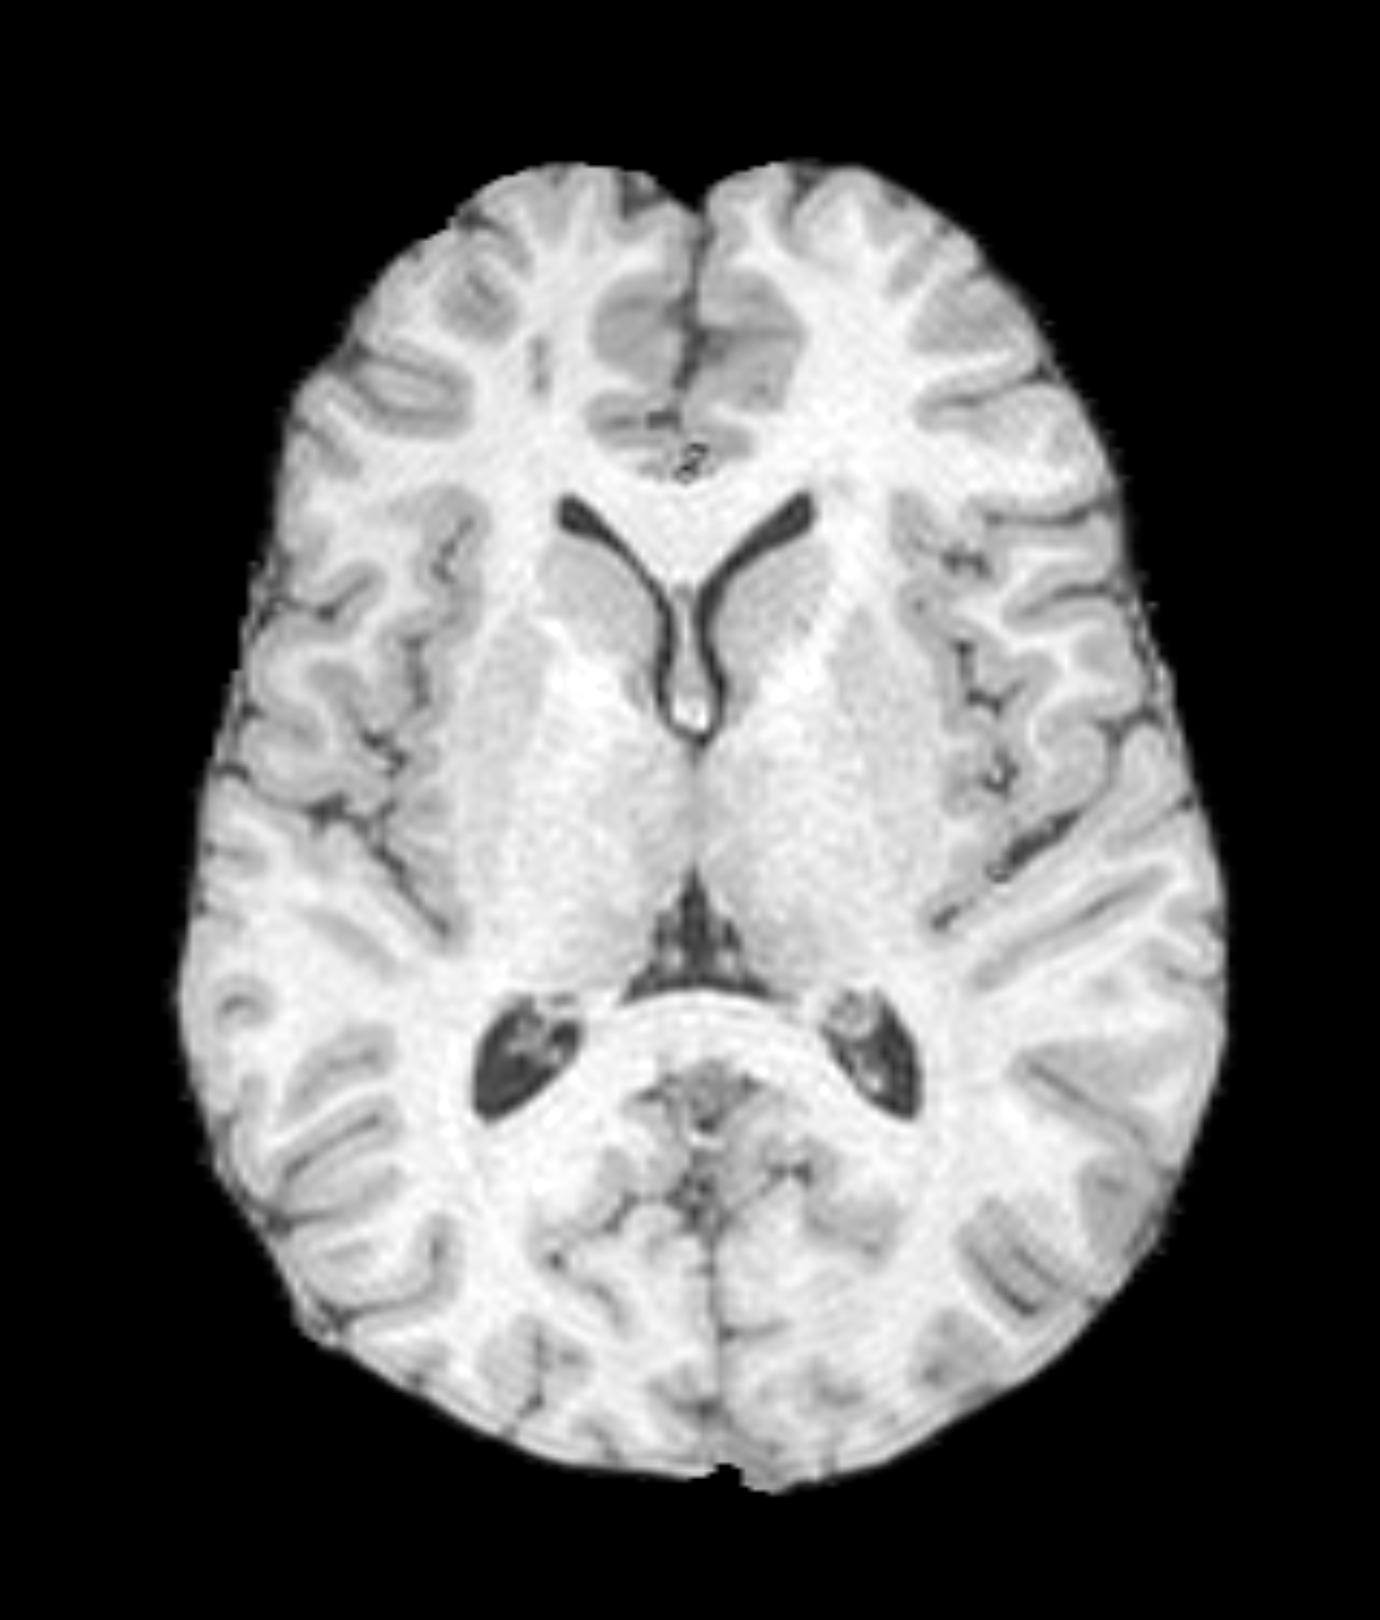
\includegraphics[scale=0.05]{./IMG/brain.jpg}
				\end{subfigure}
				\begin{subfigure}{0.99\textwidth}
					\centering
					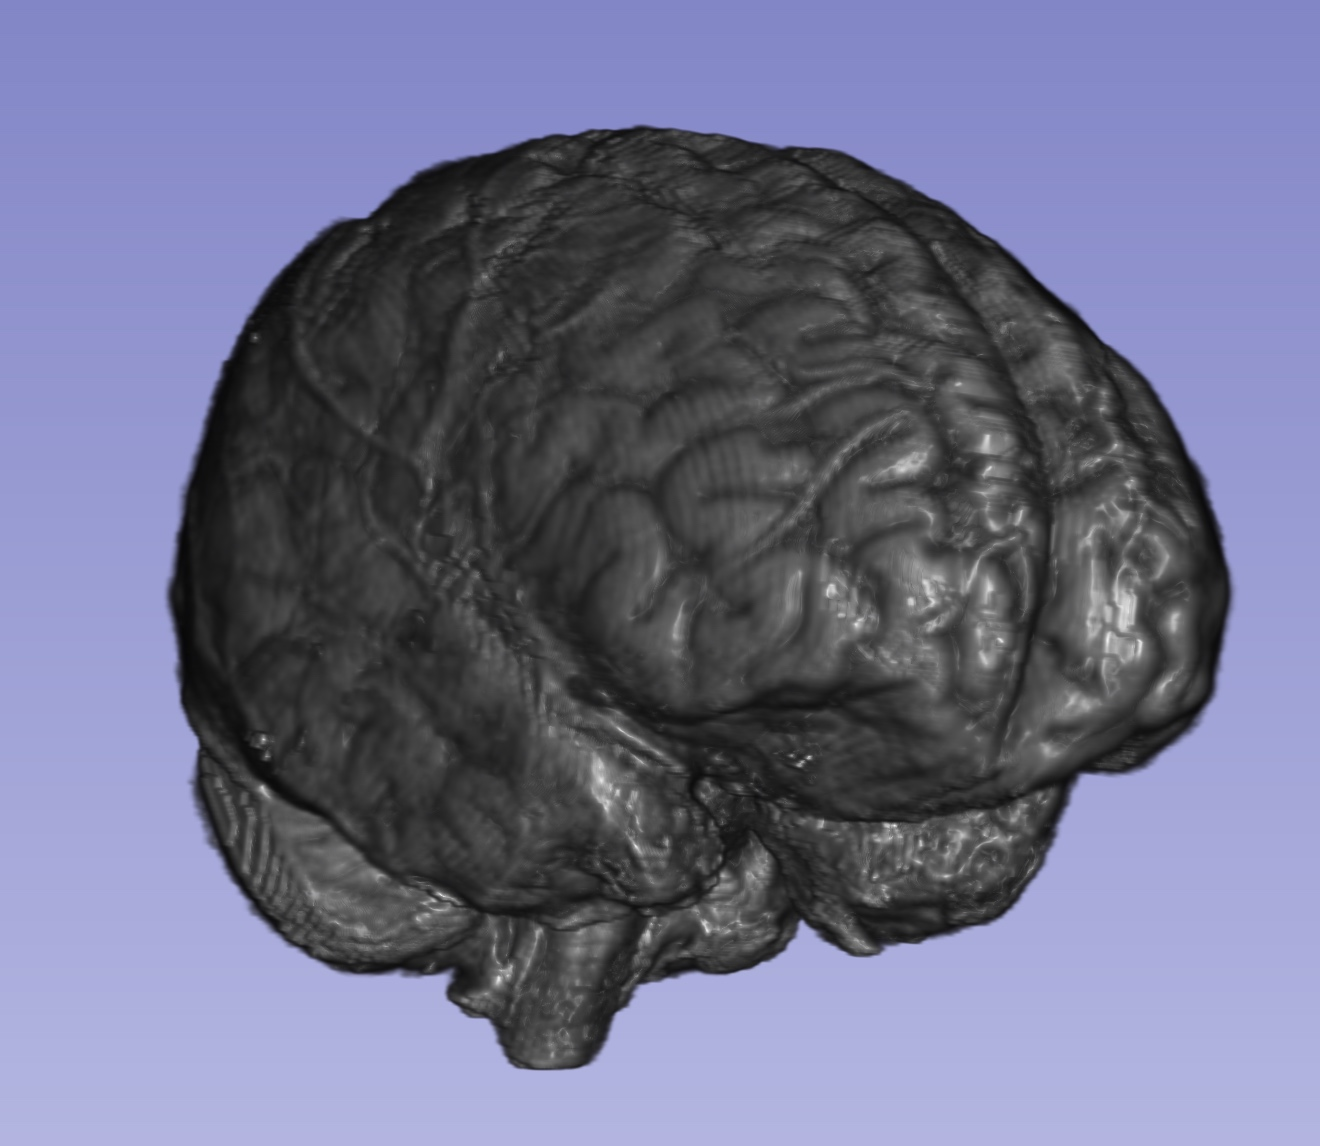
\includegraphics[scale=0.1]{./IMG/3Dbrain.jpg}
				\end{subfigure}
			\end{figure}
			\end{column}
		\end{columns}
	\end{frame}
\end{document}
